\section{Dimensionamento dei calettamenti tra alberi e ruote}
Terminato il dimensionamento degli elementi volventi, si è passati a dimensionare il calettamento tra ruote dentate ed alberi.\\
I calettamenti albero mozzo possono seguire diverse configurazioni, nel caso del riduttore in esame si è scelto l'utilizzo di profili scanalati viste le elevate potenze e coppie in gioco.\\
\\
Anche in questo caso la verifica dei singoli calettamenti è avvenuta mediante il software KissSoft. \\
\\
I profili scanalati sono caratterizzati dai parametri riportati in Fig.\ref{fig:ScanalatoGenerico}.
\begin{figure}[h]
    \centering
    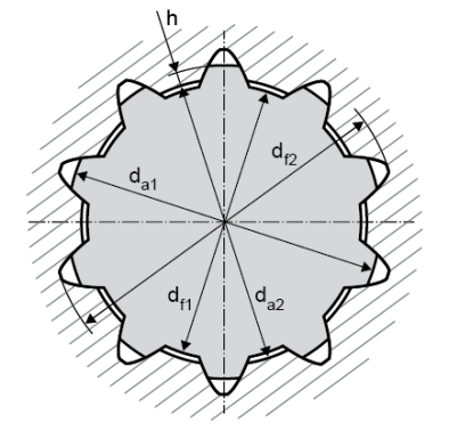
\includegraphics[scale=0.5]{Immagini/ScanalatoGenerico.png}
    \caption{Parametri caratteristici del profilo scanalato}
    \label{fig:ScanalatoGenerico}
\end{figure}

\paragraph{Profilo scanalato Albero 1 (input)}

È stato scelto un profilo scanalato caratterizzato da:
\begin{itemize}
    \item $d_{a1}=54.75$ mm;
    \item $d_{a2}=53.27$ mm;
    \item $m_a=0.75$ mm;
    \item $z=72$ (numero di denti).
\end{itemize}
\newpage
\begin{figure}[h]
    \centering
    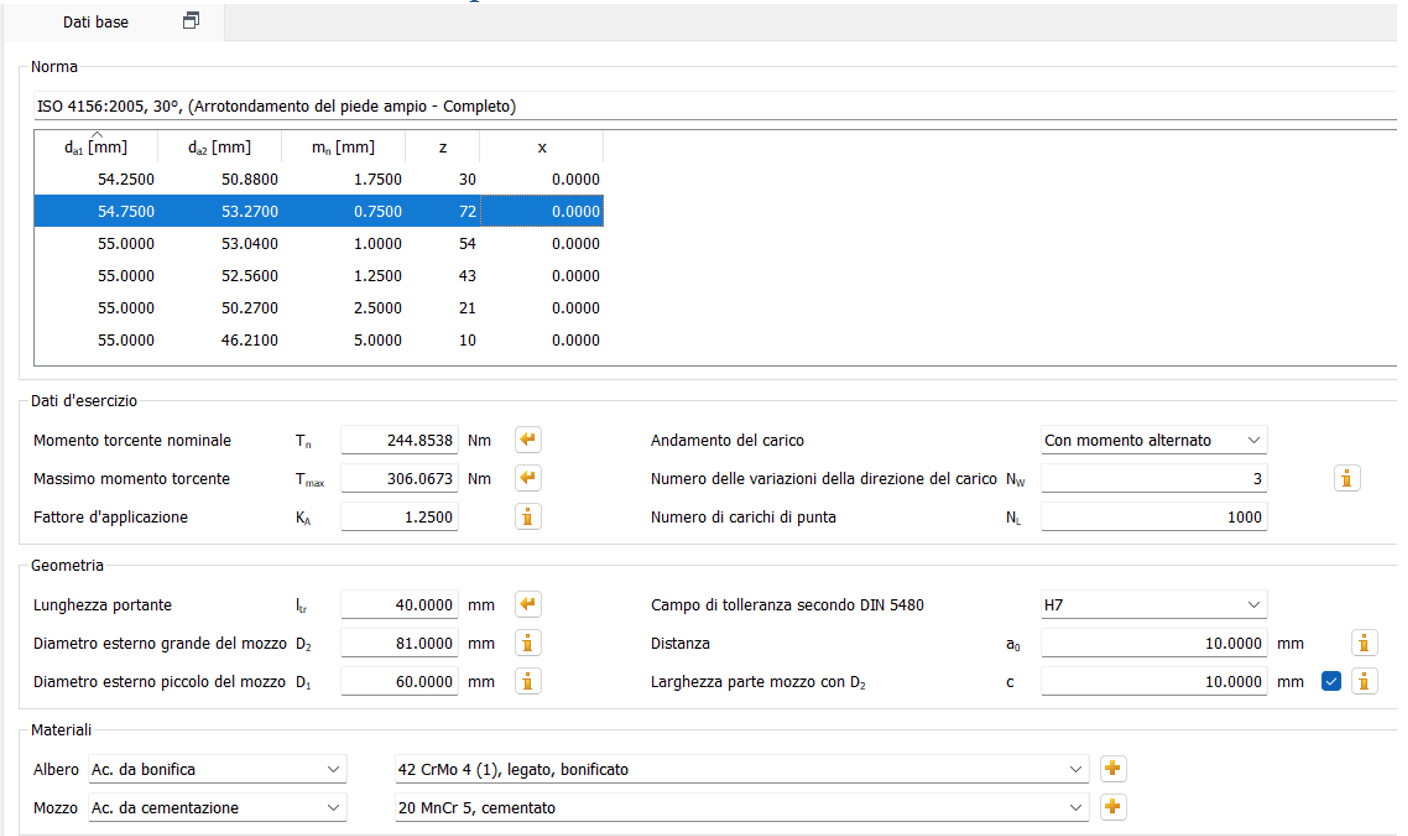
\includegraphics[scale=0.5]{Immagini/Scanalato1.png}
    \caption{Caratteristiche del profilo scanalato sull'albero 1}
    \label{fig:Scanalato1}
\end{figure}

Eseguendo il calcolo di verifica si sono ottenuti i seguenti risultati.

\emph{Albero}
\begin{figure}[h]
    \centering
    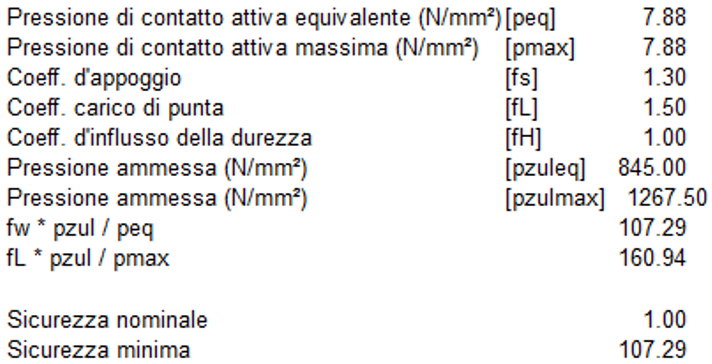
\includegraphics[scale=0.5]{Immagini/RisultatiScanalatoAlbero1.png}
    \caption{Parametri  di verifica del profilo scanalato riguardante l'albero}
    \label{fig:RisultatiScanalatoAlbero1}
\end{figure}

\emph{Mozzo}
\begin{figure}[h]
    \centering
    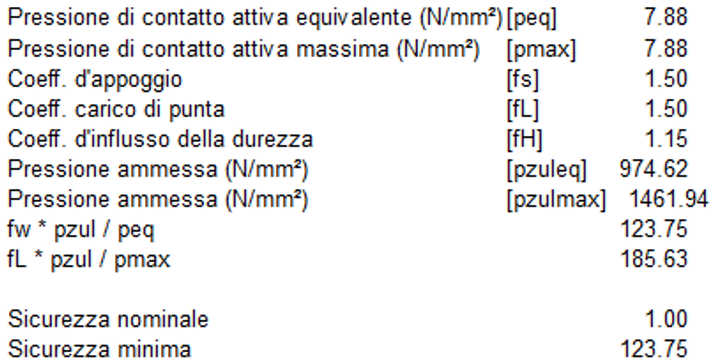
\includegraphics[scale=0.5]{Immagini/RisultatiScanalatoMozzo1.png}
    \caption{Parametri di verifica del profilo scanalato riguardante il mozzo}
    \label{fig:RisultatiScanalatoMozzo1}
\end{figure}
\newpage
In conclusione, il calettamento risulta quindi verificato nei limiti di sicurezza.
\begin{figure}[h]
    \centering
    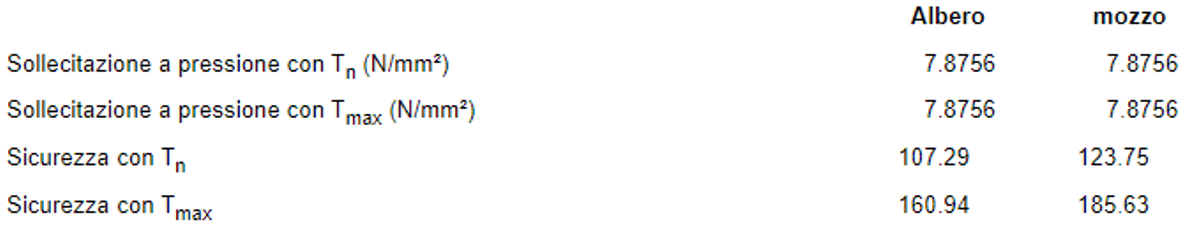
\includegraphics[scale=0.5]{Immagini/RisultatiScanalato1.png}
    \caption{Verifica del profilo scanalato dell'albero 1}
    \label{fig:RisultatiScanalato1}
\end{figure}

\paragraph{Profilo scanalato Albero 2}

È stato scelto un profilo scanalato caratterizzato da:
\begin{itemize}
    \item $d_{a1}=40$ mm;
    \item $d_{a2}=33.09$ mm;
    \item $m_a=4$ mm;
    \item $z=9$.
\end{itemize}

\begin{figure}[h]
    \centering
    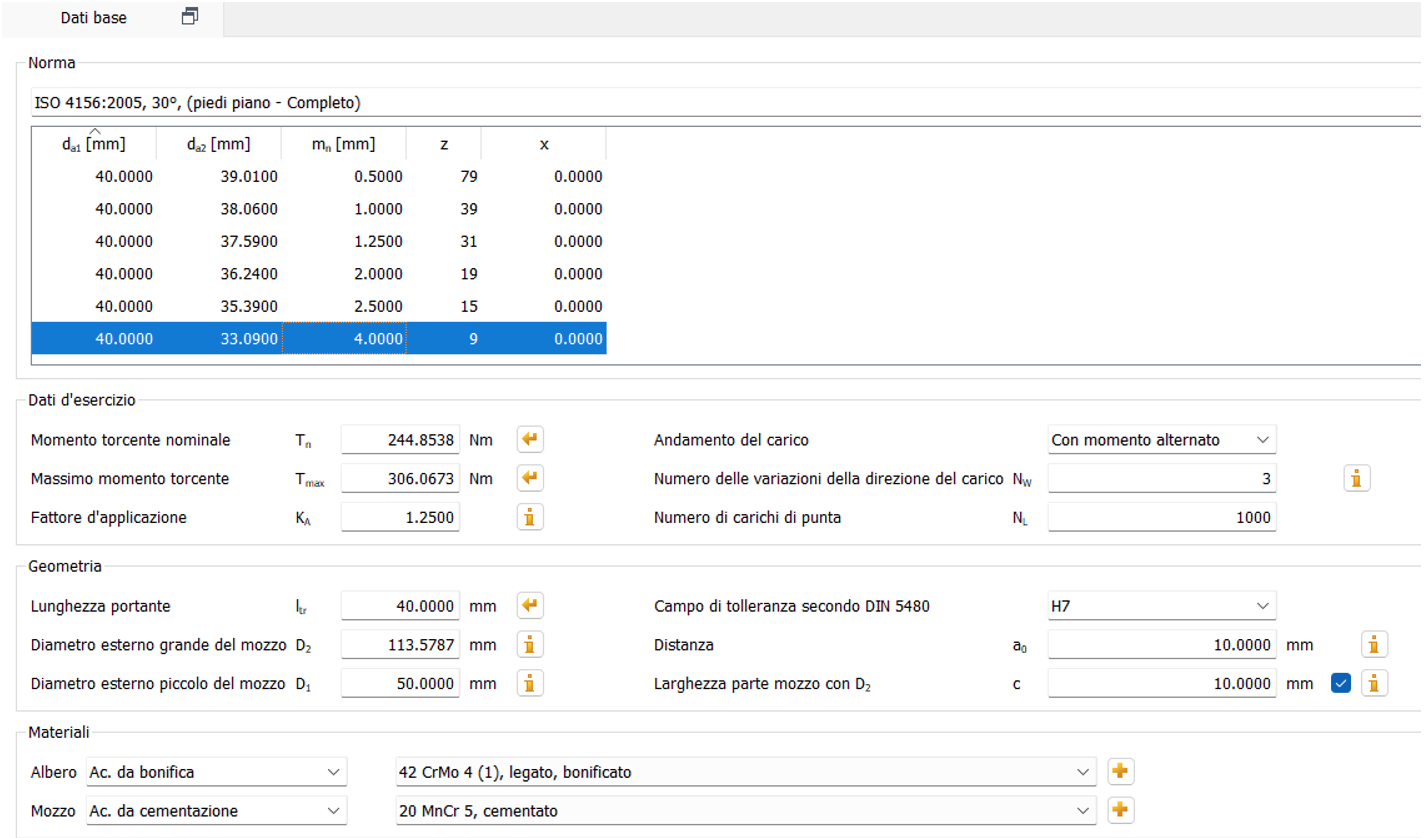
\includegraphics[scale=0.5]{Immagini/Scanalato2.png}
    \caption{Caratteristiche del profilo scanalato sull'albero 2}
    \label{fig:Scanalato2}
\end{figure}

Eseguendo il calcolo di verifica si sono ottenuti i seguenti risultati.

\emph{Albero}
\begin{figure}[h]
    \centering
    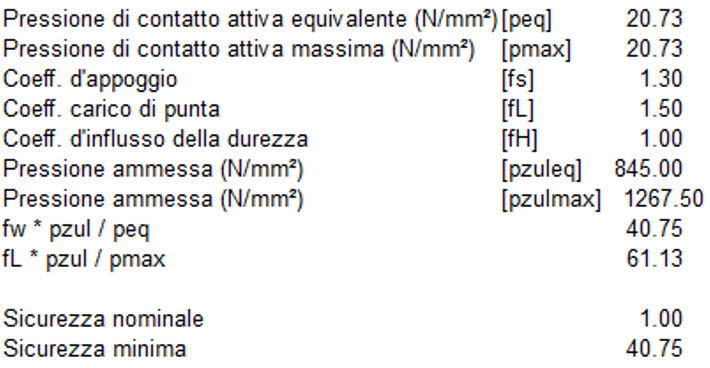
\includegraphics[scale=0.5]{Immagini/RisultatiScanalatoAlbero2.png}
    \caption{Parametri  di verifica del profilo scanalato riguardante l'albero}
    \label{fig:RisultatiScanalatoAlbero2}
\end{figure}
\newpage
\emph{Mozzo}
\begin{figure}[h]
    \centering
    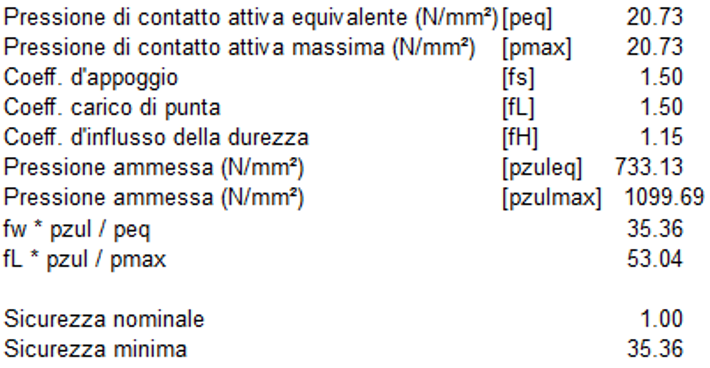
\includegraphics[scale=0.5]{Immagini/RisultatiScanalatoMozzo2.png}
    \caption{Parametri di verifica del profilo scanalato riguardante il mozzo}
    \label{fig:RisultatiScanalatoMozzo2}
\end{figure}

In conclusione, il calettamento risulta quindi verificato nei limiti di sicurezza.
\begin{figure}[h]
    \centering
    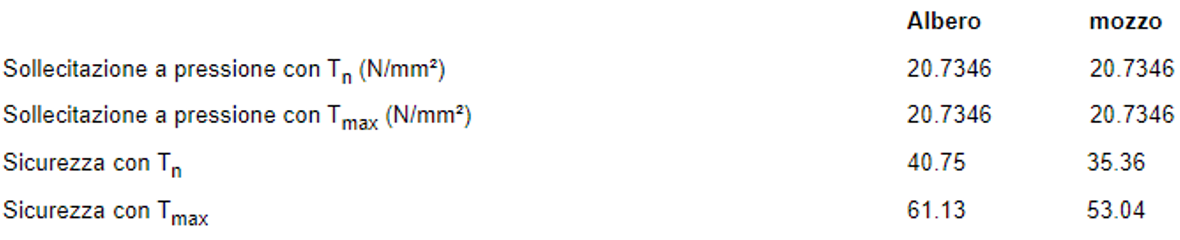
\includegraphics[scale=0.5]{Immagini/RisultatiScanalato2.png}
    \caption{Verifica del profilo scanalato dell'albero 2}
    \label{fig:RisultatiScanalato2}
\end{figure}

\paragraph{Profilo scanalato Albero 3}

È stato scelto un profilo scanalato caratterizzato da:
\begin{itemize}
    \item $d_{a1}=40$ mm;
    \item $d_{a2}=33.09$ mm;
    \item $m_a=4$ mm;
    \item $z=9$.
\end{itemize}

\begin{figure}[h]
    \centering
    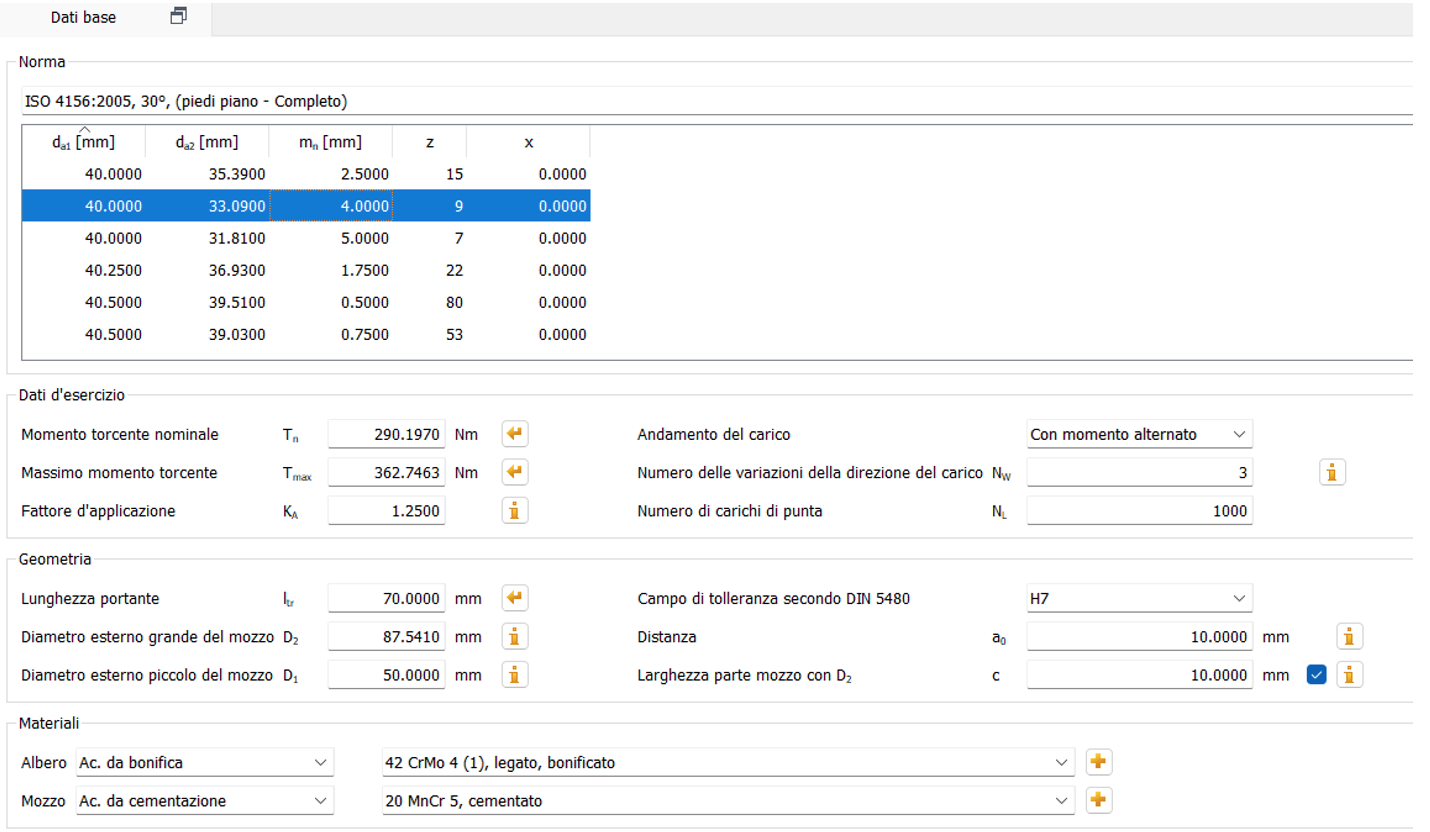
\includegraphics[scale=0.5]{Immagini/Scanalato3.png}
    \caption{Caratteristiche del profilo scanalato sull'albero 3}
    \label{fig:Scanalato3}
\end{figure}
\newpage
Eseguendo il calcolo di verifica si sono ottenuti i seguenti risultati.

\emph{Albero}
\begin{figure}[h]
    \centering
    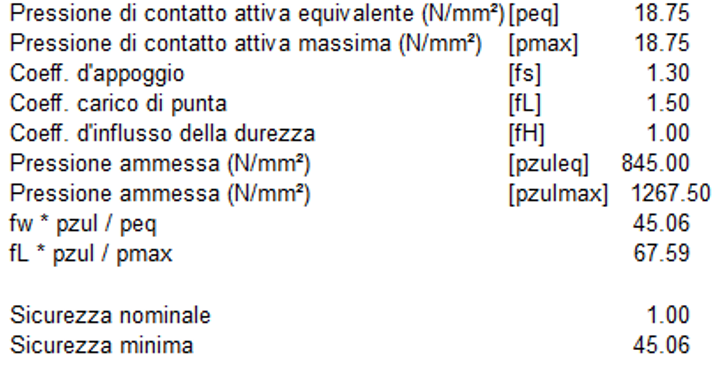
\includegraphics[scale=0.5]{Immagini/RisultatiScanalatoAlbero3.png}
    \caption{Parametri  di verifica del profilo scanalato riguardante l'albero}
    \label{fig:RisultatiScanalatoAlbero3}
\end{figure}

\emph{Mozzo}
\begin{figure}[h]
    \centering
    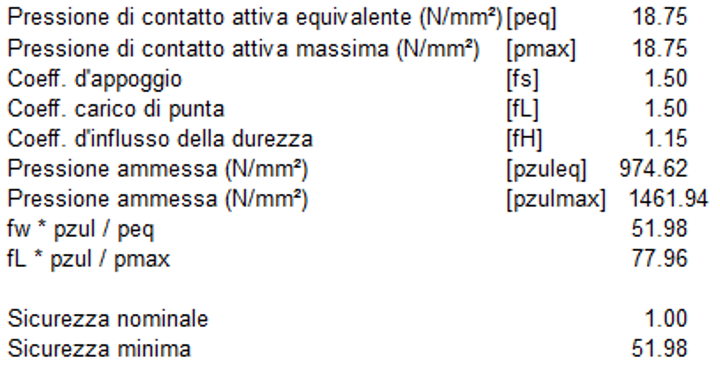
\includegraphics[scale=0.5]{Immagini/RisultatiScanalatoMozzo3.png}
    \caption{Parametri di verifica del profilo scanalato riguardante il mozzo}
    \label{fig:RisultatiScanalatoMozzo3}
\end{figure}

In conclusione, il calettamento risulta quindi verificato nei limiti di sicurezza.
\begin{figure}[h]
    \centering
    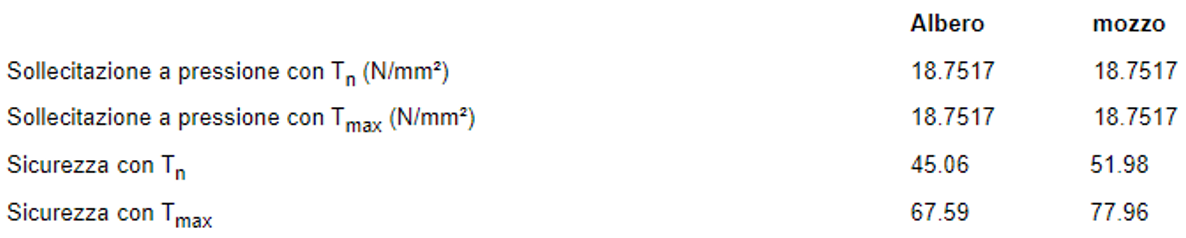
\includegraphics[scale=0.5]{Immagini/RisultatiScanalato3.png}
    \caption{Verifica del profilo scanalato dell'albero 3}
    \label{fig:RisultatiScanalato3}
\end{figure}

\paragraph{Profilo scanalato Albero 4}

È stato scelto un profilo scanalato caratterizzato da:
\begin{itemize}
    \item $d_{a1}=44.5$ mm;
    \item $d_{a2}=40$ mm;
    \item $m_a=2.5$ mm;
    \item $z=16$.
\end{itemize}
\newpage
\begin{figure}[h]
    \centering
    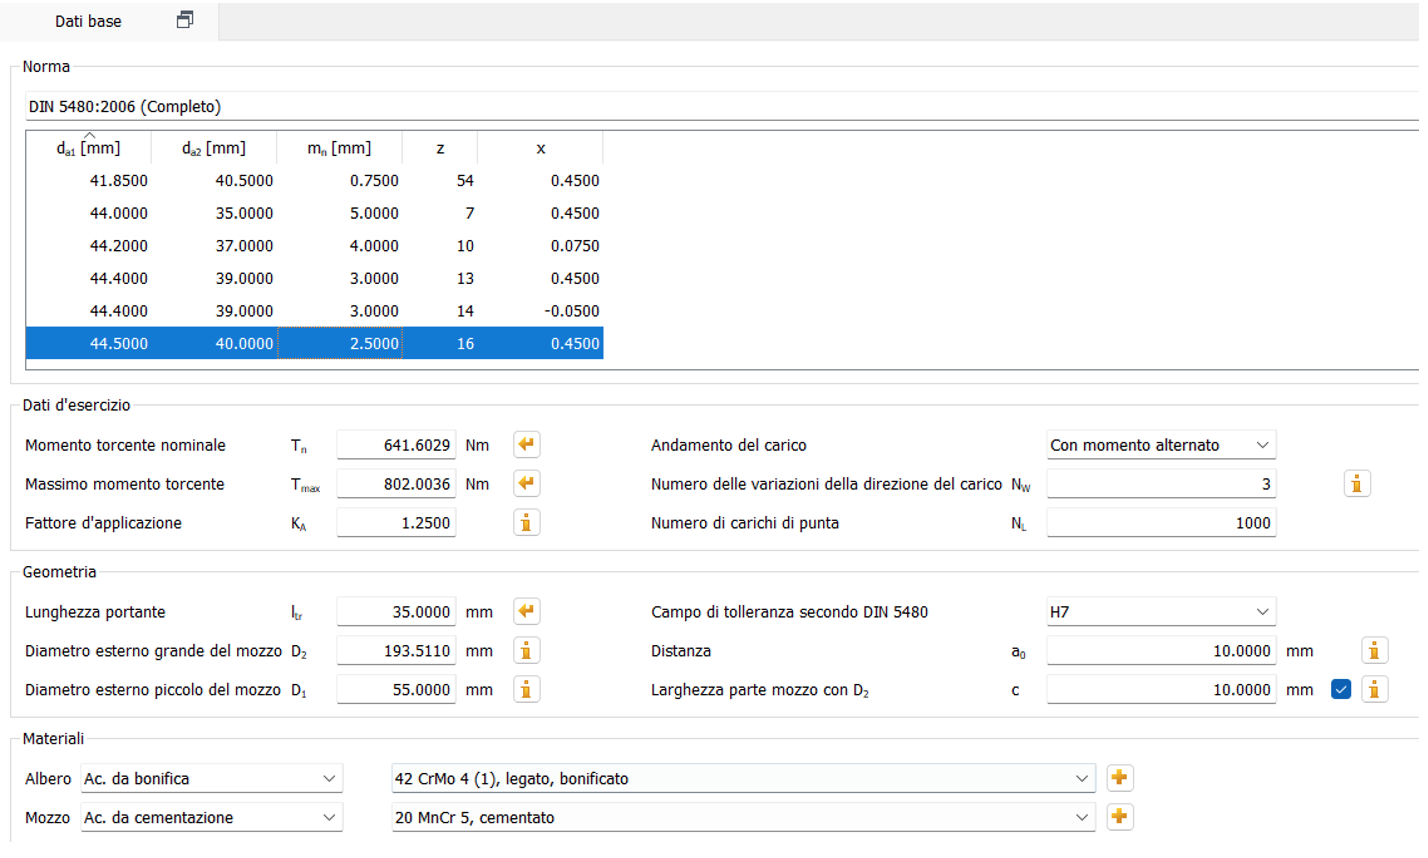
\includegraphics[scale=0.5]{Immagini/Scanalato4.png}
    \caption{Caratteristiche del profilo scanalato sull'albero 4}
    \label{fig:Scanalato4}
\end{figure}

Eseguendo il calcolo di verifica si sono ottenuti i seguenti risultati.

\emph{Albero}
\begin{figure}[h]
    \centering
    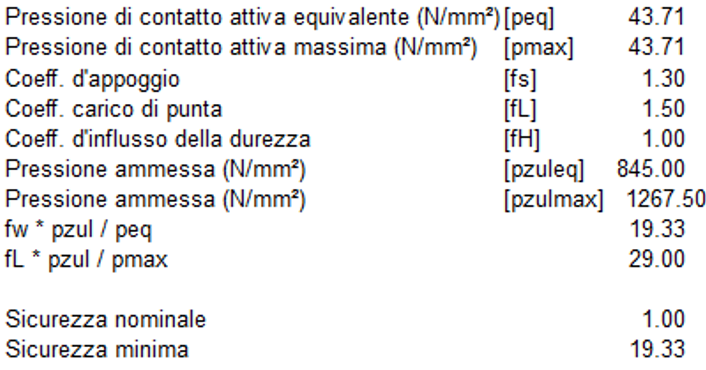
\includegraphics[scale=0.5]{Immagini/RisultatiScanalatoAlbero4.png}
    \caption{Parametri  di verifica del profilo scanalato riguardante l'albero}
    \label{fig:RisultatiScanalatoAlbero4}
\end{figure}

\emph{Mozzo}
\begin{figure}[h]
    \centering
    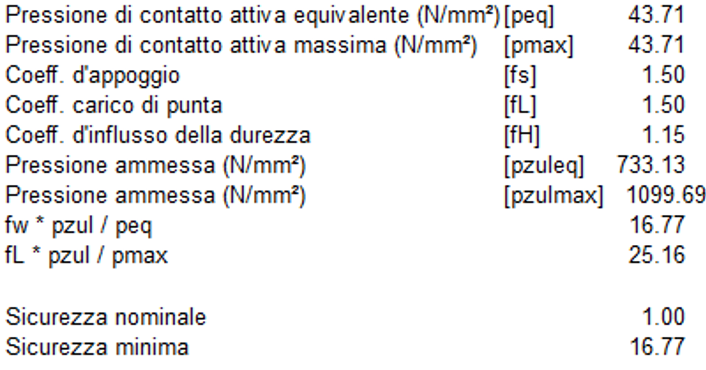
\includegraphics[scale=0.5]{Immagini/RisultatiScanalatoMozzo4.png}
    \caption{Parametri di verifica del profilo scanalato riguardante il mozzo}
    \label{fig:RisultatiScanalatoMozzo4}
\end{figure}
\newpage
In conclusione, il calettamento risulta quindi verificato nei limiti di sicurezza.
\begin{figure}[h]
    \centering
    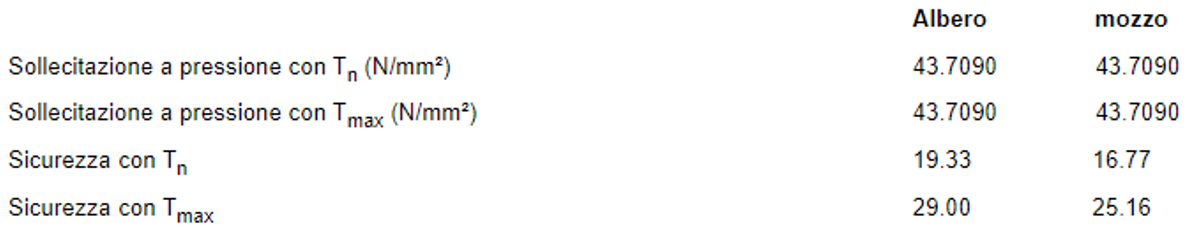
\includegraphics[scale=0.5]{Immagini/RisultatiScanalato4.png}
    \caption{Verifica del profilo scanalato dell'albero 4}
    \label{fig:RisultatiScanalato4}
\end{figure}

\paragraph{Profilo scanalato Albero 5}

È stato scelto un profilo scanalato caratterizzato da:
\begin{itemize}
    \item $d_{a1}=41.25$ mm;
    \item $d_{a2}=38.84$ mm;
    \item $m_a=1.25$ mm;
    \item $z=32$.
\end{itemize}

\begin{figure}[h]
    \centering
    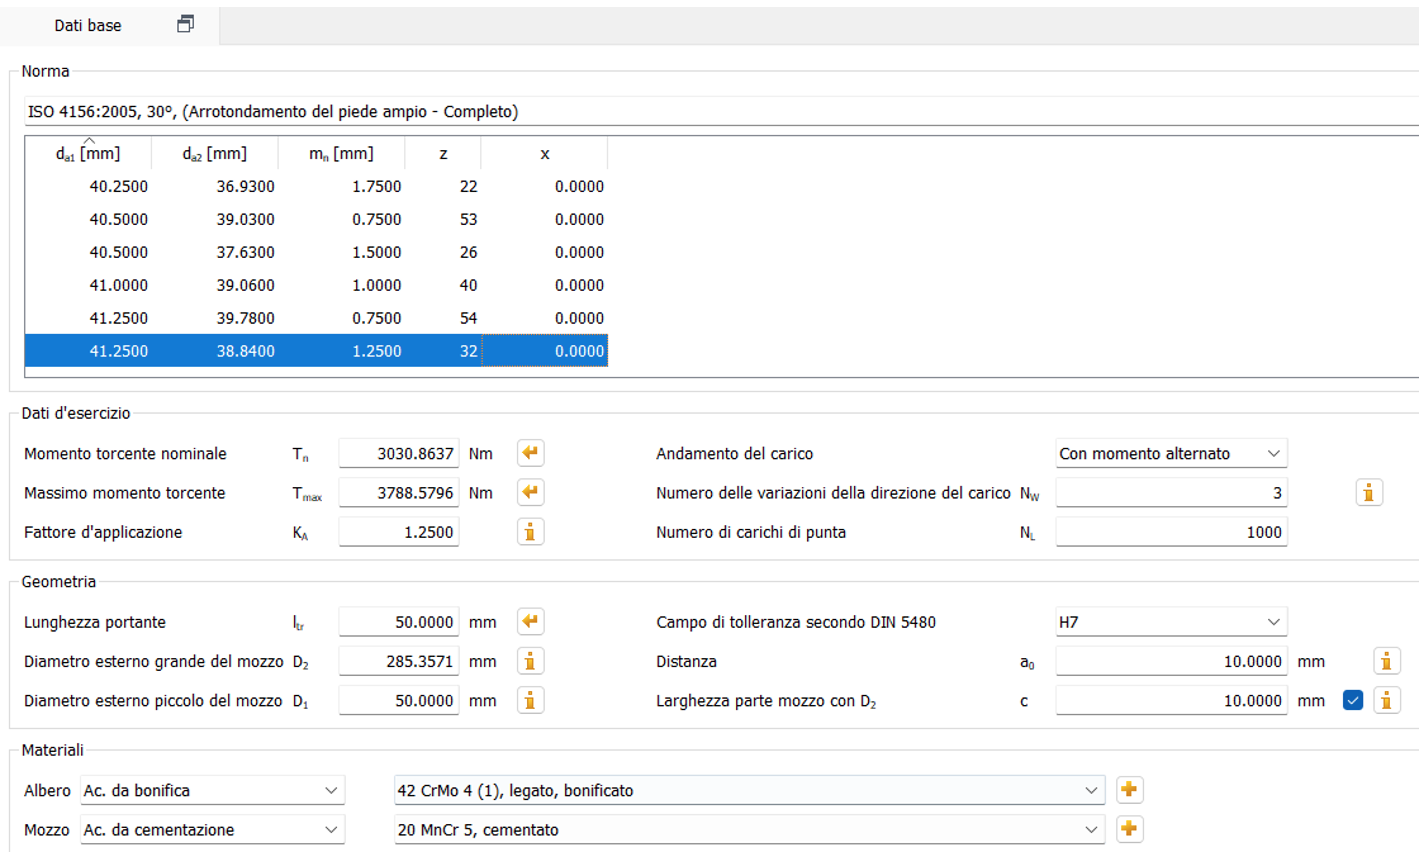
\includegraphics[scale=0.5]{Immagini/Scanalato5.png}
    \caption{Caratteristiche del profilo scanalato sull'albero 5}
    \label{fig:Scanalato5}
\end{figure}

Eseguendo il calcolo di verifica si sono ottenuti i seguenti risultati.

\emph{Albero}
\begin{figure}[h]
    \centering
    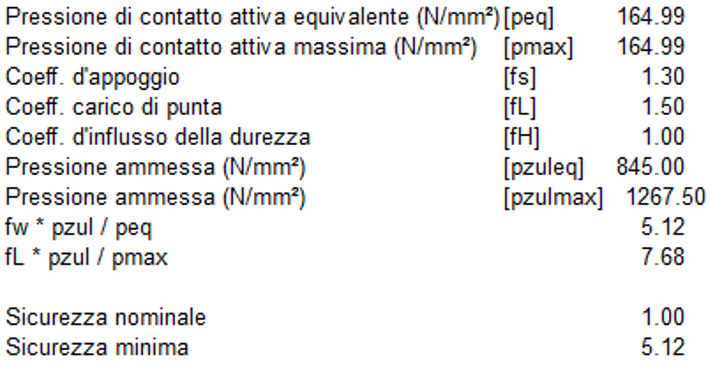
\includegraphics[scale=0.5]{Immagini/RisultatiScanalatoAlbero5.png}
    \caption{Parametri  di verifica del profilo scanalato riguardante l'albero}
    \label{fig:RisultatiScanalatoAlbero5}
\end{figure}
\newpage
\emph{Mozzo}
\begin{figure}[h]
    \centering
    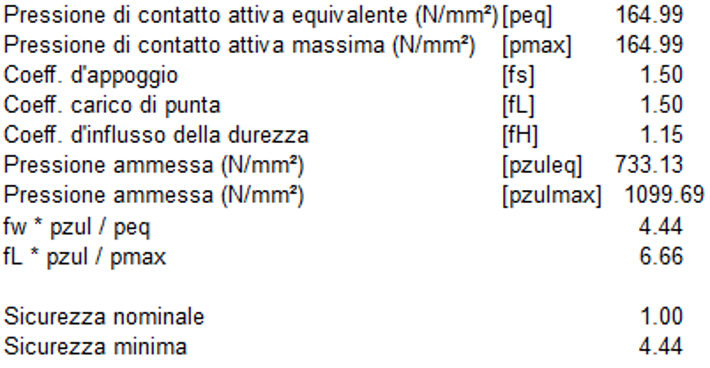
\includegraphics[scale=0.5]{Immagini/RisultatiScanalatoMozzo5.png}
    \caption{Parametri di verifica del profilo scanalato riguardante il mozzo}
    \label{fig:RisultatiScanalatoMozzo5}
\end{figure}

In conclusione, il calettamento risulta quindi verificato nei limiti di sicurezza.
\begin{figure}[h]
    \centering
    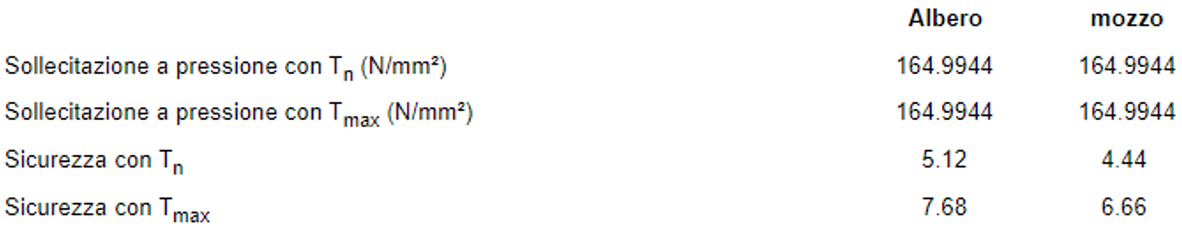
\includegraphics[scale=0.5]{Immagini/RisultatiScanalato5.png}
    \caption{Verifica del profilo scanalato dell'albero 5}
    \label{fig:RisultatiScanalato5}
\end{figure}
